\documentclass[14pt]{beamer}
%\documentclass[14pt, handout]{beamer} %Makes Handouts
\usetheme{Singapore} %Gray with fade at top
\useoutertheme[subsection=false]{miniframes} %Supppress subsection in header
\useinnertheme{rectangles} %Itemize/Enumerate boxes
\usecolortheme{seagull} %Color theme
\usecolortheme{rose} %Inner color theme

\definecolor{light-gray}{gray}{0.75}
\definecolor{dark-gray}{gray}{0.55}
\setbeamercolor{item}{fg=light-gray}
\setbeamercolor{enumerate item}{fg=dark-gray}

\setbeamertemplate{navigation symbols}{}
\setbeamertemplate{mini frames}{}
%\setbeamercovered{dynamics}
\setbeamerfont*{title}{size=\Large,series=\bfseries}
\setbeamerfont{footnote}{size=\tiny}

%\setbeameroption{notes on second screen} %Dual-Screen Notes
%\setbeameroption{show only notes} %Notes Output

\setbeamertemplate{frametitle}{\vspace{.5em}\bfseries\insertframetitle}
\newcommand{\heading}[1]{\noindent \textbf{#1}\\ \vspace{1em}}
\newcommand{\questions}{\frame{\vspace{4em}\centering{\Large Questions?}}}
\newcommand{\Ractivity}[1]{\frame{\vspace{4em}\centering{\Large Let's work in R!\\ \vspace{1em} {(#1)}}}}


\usepackage{bbding,color,multirow,times,ccaption,tabularx,graphicx,verbatim,booktabs}
\usepackage{colortbl} %Table overlays
\usepackage[english]{babel}
\usepackage[latin1]{inputenc}
\usepackage[T1]{fontenc}
\usepackage{lmodern}
\usepackage{alltt}

\usepackage{tikz}
\usetikzlibrary{shapes,arrows,decorations.pathreplacing,calc}


\author[]{Thomas J. Leeper}
\institute{
  Government Department\\London School of Economics and Political Science
}


\title{Experimental Research in Legislative Studies}

\date[]{18 August 2017}

\begin{document}

\frame{\titlepage}


\frame{

\frametitle{Activity!}

\only<2-4,6>{
\begin{enumerate}
\item<2-4,6> Ask you to guess a number
\item<3-4,6> Number off 1 and 2 across the room
\item<4,6> Group 2, close your eyes
\item<6> Group 1, close your eyes
\end{enumerate}
}

\Large
\only<5>{\textit{Group 1}\\ Think about whether the population of Chicago is more or less than 500,000 people. What do you think the population of Chicago is?}
\only<7>{\textit{Group 2}\\ Think about whether the population of Chicago is more or less than 10,000,000 people. What do you think the population of Chicago is?}

}
\frame{}

\frame{

\frametitle{Enter your data}

\begin{itemize}\itemsep1em
\item Go here: \url{http://bit.ly/297vEdd}
\item Enter your guess and your group number
\end{itemize}

%http://goo.gl/forms/xDW4FLm9pau0O8zz2

}


\frame{

\frametitle{Results}

\begin{itemize}\itemsep1em
\item True population: 2.79 million
\item<2-> What did you guess? \href{https://docs.google.com/spreadsheets/d/1SKWljS1EeNkAV5V0NZUwrKOu3LQFILVMB37xfTxyrPM/edit?usp=sharing}{(See Responses)}
\item<3-> What's going on here?
	\begin{itemize}
	\item An experiment!
	\item Demonstrates ``anchoring'' heuristic
	\end{itemize}
\item<4-> Experiments are easy to analyze and generate causal inferences, but only if designed and implemented well
\end{itemize}

}

\frame{\tableofcontents[subsubsectionstyle=hide]}

\frame{
\frametitle{Who am I?}

\small

\begin{itemize}\itemsep0.25em

\item Thomas Leeper

\item Associate Professor in Political Behaviour at London School of Economics

\begin{itemize}
\item 2013--15: Aarhus University (Denmark)
\item 2008--12: PhD from Northwestern University (Chicago, USA)
\item Birth--2008: Minnesota, USA
\end{itemize}

\item Interested in survey and experimental methods and political psychology

\item Email: \href{mailto:t.leeper@lse.ac.uk}{t.leeper@lse.ac.uk}

\end{itemize}

}


\frame{

\frametitle{Who are you?}

\begin{itemize}\itemsep1em

\item What's your name?

\item Where are you from?

\item Have you designed and/or analyzed an experiment before?

\end{itemize}

}


\frame{

\frametitle{Course Materials}

\begin{center}
All material for this workshop, including required and suggested readings, are available at:\\

\vspace{1em}

\url{http://www.thomasleeper.com/legexpcourse/}
\end{center}

}

\frame[label=learningoutcomes]{

\frametitle{Learning Outcomes}

\small

By the end of the day, you should be able to\dots

\begin{enumerate}
\item<2-> Explain how to analyze experiments quantitatively.
\item<3-> Explain how to design experiments that speak to relevant research questions and theories.
\item<4-> Evaluate the uses and limitations of three common legislative experimental paradigms: survey experiments, field experiments, and simulations.
\item<5-> Identify practical issues that arise in the implementation of experiments and evaluate how to anticipate and respond to them.
\end{enumerate}

}

\frame{\tableofcontents}


\questions


\section{Causal Inference}
\frame{\tableofcontents[currentsection]}


\frame{

\frametitle{Experiments: Definition}

Oxford English Dictionary defines ``experiment'' as:\\

\begin{enumerate}\itemsep1em
\item A scientific procedure undertaken to make a discovery, test a hypothesis, or demonstrate a known fact
\item A course of action tentatively adopted without being sure of the outcome
\end{enumerate}
}

\frame{

\frametitle{Experiments have a long history}

\begin{itemize}\itemsep0.75em
\item Origins in agricultural and biostatistical research in the 19th century (Fisher, Neyman, Pearson, etc.)

\item First randomized, controlled trial (RCT) by Peirce and Jastrow in 1884

\item First polisci experiment by Gosnell (1924)

\item Survey experiments have been common since 1930s

\item Gerber and Green (2000) first \textit{major}, \textit{modern}, \textit{field} experiment

\end{itemize}

}


\frame{

\frametitle{Legislative Experiments}

\small

\begin{itemize}\itemsep0.5em
\item Experiments in legislative contexts fit awkwardly in that history and the dominant paradigms have very different histories

\item<2-> \textbf{Simulations}
	
	\begin{itemize}
	\item Originated in formal literatures on committee behavior, coalition formation, and majority rule institutions
	\end{itemize}

\item<3-> \textbf{Field experiments}

	\begin{itemize}
	\item Really only emerged in the past decade
	\end{itemize}

\item<4-> \textbf{Survey Experiments}

	\begin{itemize}
	\item Much more sparsely used for reasons that will become obvious
	\end{itemize}
\end{itemize}

}


\frame{}

\frame{

\frametitle{{\normalsize What kinds of questions can we answer with experiments?}}

\normalsize

\begin{itemize}\itemsep1em
\item<2-> Forward causal questions
	\begin{itemize}
	\item Can X cause Y?
	\item What effects does X have?
	\end{itemize}
\item<3-> Backward causal questions
	\begin{itemize}
	\item What causes Y?
	\item How much of Y is attributable to X?
	\end{itemize}
\item<4-> Even though answering ``forward'' causal question, we start with an outcome concept
\end{itemize}
}


% Causal graphs
\begin{frame}
\begin{center}
\begin{tikzpicture}[>=latex',circ/.style={draw, shape=circle, node distance=5cm, line width=1.5pt}]
    \draw (0,0) node[left] (X) {\textcolor<2->{red}{Smoking}};
    \draw[->] (X) -- (5,0) node[right] (Y) {Cancer};
    \draw[->] (-3,3) node[above] (Z) {Sex} -- (X);
    \draw[->] (Z) -- (Y);
    \draw[->] (5,2) node[above] (A) {Environment} -- (Y);
    \draw[->] (4,-3) node[below, text width=3cm, align=center] (E) {Genetic\\Predisposition} -- (Y);
    \draw[->] (-2, -2) node[below, text width=2.5cm, align=center] (W) {Parental\\Smoking} -- (X);
    \draw[->] (W) -- (Y);
    \draw<2->[->, dashed, very thick] (E) -- (X);
\end{tikzpicture}
\end{center}
\end{frame}


\frame{

\frametitle{Principles of causality}

\begin{enumerate}\itemsep1em
\item \textbf<2->{Correlation/Relationship}
\item \textbf<2->{Nonconfounding}
\item \textbf<2->{Direction (``temporal precedence'')}

\vspace{1em}

\item Mechanism

\vspace{0.5em}

\item Appropriate level of analysis
\end{enumerate}
}


\frame{

\frametitle{Establishing Relationship}

\begin{itemize}\itemsep1em
\item This is fairly trivial
\item Simply find value of $Corr(X,Y)$
\item In causal inference we often talk about correlations in terms of \textit{differences}
	\begin{itemize}
	\item Difference in values of $Y$ across values of $X$
	\item The presence of a difference indicates a correlation
	\end{itemize}
\end{itemize}

}

\frame{

\frametitle{Addressing Confounding}

In observational studies, we address confounding by:

\begin{enumerate}\itemsep1em
\item<2-> Correlating a ``putative'' cause ($X$) and an outcome ($Y$)
\item<3-> Identifying all possible confounds (\textbf{Z})
\item<4-> ``Conditioning'' on all confounds
	\begin{itemize}
	\item Calculating correlation between $X$ and $Y$ at each combination of levels of \textbf{Z}
	\end{itemize}
\end{enumerate}

}

\frame{

\frametitle{Temporal Precedence}

\begin{itemize}\itemsep0.5em
\item Even if an observational design identifies a relationship and credibly addresses sources of confounding, it still may not be a credible causal inference

\item<2-> ``Reverse causality'' is vague, referring to:
	\begin{itemize}
	\item Ambiguity about causal ordering, or
	\item Sequentially reinforcing causality between $X$ and $Y$
	\end{itemize}

\item<3-> Causation is strictly forward moving in time

\item<4-> $X$ must precede $Y$ in time for $X$ to cause $Y$

	\begin{itemize}
	\item $X$ can be \textit{measured} after $Y$ as long as it comes before it
	\end{itemize}
	
\end{itemize}

}


\frame{
\begin{center}
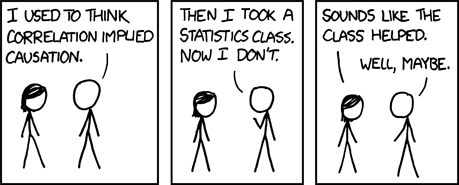
\includegraphics[width=0.95\textwidth]{images/xkcdcorrelation}
\end{center}
}



\frame{

\frametitle{Experiments!}

\begin{itemize}\itemsep0.75em
\item<2-> A randomized experiment, or randomized control trial (RCT) is:
\end{itemize}
	\begin{quote}\small
		The observation of units after, and possibly before, a randomly assigned intervention in a controlled setting, which tests one or more precise causal expectations
	\end{quote}
\begin{itemize}\itemsep0.75em
\item<3-> If we manipulate the thing we want to know the effect of ($X$), and control (i.e., hold constant) everything we do not want to know the effect of ($Z$), the only thing that can affect the outcome ($Y$) is $X$.
\end{itemize}

}

\begin{frame}
\small 
\begin{center}
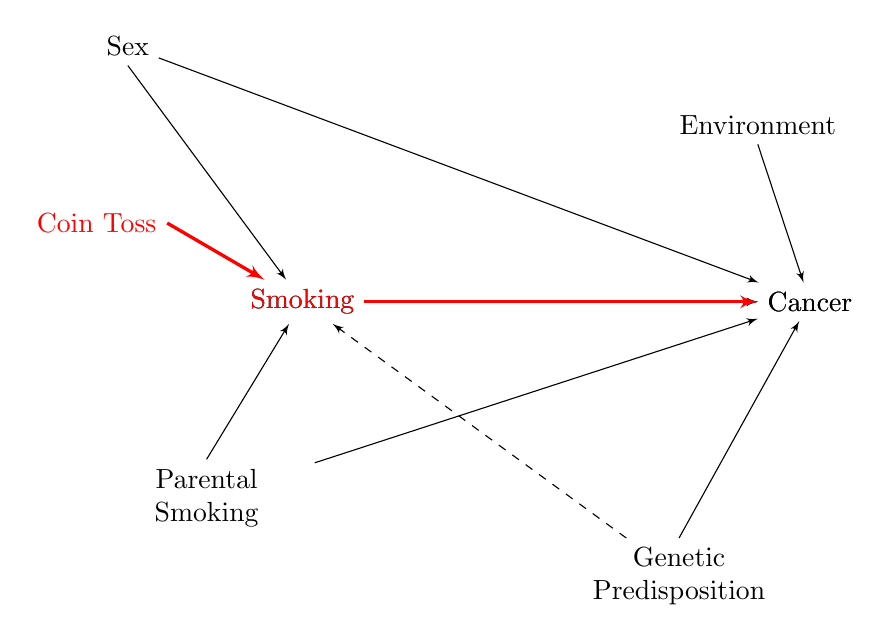
\begin{tikzpicture}[>=latex',circ/.style={draw, shape=circle, node distance=5cm, line width=1.5pt}]
    \draw<1>[->] (0,0) node[left] (X) {Smoking} -- (5,0) node[right] (Y) {Cancer};
    \draw<2>[->] (0,0) node[left, color=red] (X) {Smoking} -- (5,0) node[right] (Y) {Cancer};
    \draw[->] (-3,3) node[above] (Z) {Sex} -- (X);
    \draw[->] (Z) -- (Y);
    \draw[->] (5,2) node[above] (A) {Environment} -- (Y);
    \draw[->] (4,-3) node[below, text width=3cm, align=center] (E) {Genetic\\Predisposition} -- (Y);
    \draw[->] (-2, -2) node[below, text width=2.5cm, align=center] (W) {Parental\\Smoking} -- (X);
    \draw[->] (W) -- (Y);
    \draw[->, dashed] (E) -- (X);
    
    \draw<2->[->, very thick, color=red] (-2.5,1) node[left, color=red] (Tr) {Coin Toss} -- (X);
    \draw<2->[->, very thick, color=red] (X) -- (Y);
\end{tikzpicture}
\end{center}
\end{frame}


\questions


\frame{

\frametitle{Definitions}

\only<2>{\textbf{Unit}: A physical object at a particular point in time}

\only<3>{\textbf{Treatment}: An intervention, whose effect(s) we wish to assess relative to some other (non-)intervention}

\only<4>{\textbf{Outcome}: The variable we are trying to explain}

\only<5>{
\textbf{Potential outcomes}: The outcome value for each unit that we \textit{would observe} if that unit received each treatment\\

\vspace{1em}

Multiple potential outcomes for each unit, but we only observe one of them

}

\only<6>{\textbf{Causal effect}: The comparisons between the unit-level potential outcomes under each intervention\\

\vspace{1em}

\textit{This is what we want to know!}
}

}

\frame{
	\frametitle{``The Perfect Doctor''}

\small
\begin{center}
\begin{tabular}{ccc}
Unit & $Y_0$ & $Y_1$ \\ \hline 
1 & ? & ? \\
2 & ? & ? \\
3 & ? & ? \\
4 & ? & ? \\
5 & ? & ? \\
6 & ? & ? \\
7 & ? & ? \\
8 & ? & ? \\ \hline
\textbf{Mean} & \textbf{?} & \textbf{?} \\
\end{tabular}
\end{center}
}

\frame{
	\frametitle{``The Perfect Doctor''}

\small
\begin{center}
\begin{tabular}{ccc}
Unit & $Y_0$ & $Y_1$ \\ \hline 
1 & ? & 14 \\
2 & 6 & ? \\
3 & 4 & ? \\
4 & 5 & ? \\
5 & 6 & ? \\
6 & 6 & ? \\
7 & ? & 10 \\
8 & ? & 9 \\ \hline
\textbf{Mean} & \textbf{5.4} & \textbf{11} \\
\end{tabular}
\end{center}
}

\frame{
	\frametitle{``The Perfect Doctor''}

\small
\begin{center}
\begin{tabular}{ccc}
Unit & $Y_0$ & $Y_1$ \\ \hline 
1 & 13 & 14 \\
2 & 6 & 0 \\
3 & 4 & 1 \\
4 & 5 & 2 \\
5 & 6 & 3 \\
6 & 6 & 1 \\
7 & 8 & 10 \\
8 & 8 & 9 \\ \hline
\textbf{Mean} & \textbf{7} & \textbf{5} \\
\end{tabular}
\end{center}
}



\frame{
	\frametitle{Experimental Inference I}
	\begin{itemize}\itemsep1em
    	\item<1-> We cannot see individual-level causal effects
    	\item<2-> We can see \textit{average causal effects}
    		\begin{itemize}
        		\item<2-> Ex.: Average difference in cancer between those who do and do not smoke
    		\end{itemize}
    	\item<3-> We want to know: $TE_i = Y_{1i} - Y_{0i}$
	\end{itemize}
}

\frame{
	\frametitle{Experimental Inference II}
	\begin{itemize}\itemsep1em
		\item<1-> We want to know: $TE_i = Y_{1i} - Y_{0i}$
		\item<2-> We can average: $ATE = E[Y_{1i} - Y_{0i}] = E[Y_{1i}] - E[Y_{0i}]$
		\item<3-> But we still only see one potential outcome for each unit:\\ \vspace{1em}
    		$ATE_{naive} = E[Y_{1i} | X = 1] - E[Y_{0i} | X = 0]$
    	\item<4-> Is this what we want to know?
	\end{itemize}
}


\frame{
	\frametitle{Experimental Inference III}
	\small
	\begin{itemize}\itemsep1em
	\item What we want and what we have:
		\begin{align}
		ATE & = E[Y_{1i}] - E[Y_{0i}] \\[1em]
		ATE_{naive} & = E[Y_{1i} | X = 1] - E[Y_{0i} | X = 0]
		\end{align}		
	\item<2-> Are the following statements true?\\
  		\begin{itemize}\itemsep0.5em
      		\item<2-> $E[Y_{1i}] = E[Y_{1i} | X = 1]$
      		\item<2-> $E[Y_{0i}] = E[Y_{0i} | X = 0]$
  		\end{itemize}
  	\item<3-> Not in general!
  	\end{itemize}
}

\frame{
	\frametitle{Experimental Inference IV}
	\small
	\begin{itemize}\itemsep0.5em
    	\item Only true when both of the following hold:
    	\begin{align}
    	E[Y_{1i}] = E[Y_{1i} | X = 1] = E[Y_{1i} | X = 0]\\
    	E[Y_{0i}] = E[Y_{0i} | X = 1] = E[Y_{0i} | X = 0]
    	\end{align}
    	\item In that case, potential outcomes are \textit{independent} of treatment assignment
		\item If true, then:
    	\begin{align*}
    	ATE_{naive} & = E[Y_{1i} | X = 1] - E[Y_{0i} | X = 0] \tag{5}\\
    	& = E[Y_{1i}] - E[Y_{0i}]\\
    	& = ATE
    	\end{align*}
	\end{itemize}
}

\frame{
	\frametitle{Experimental Inference V}
	\small
	\begin{itemize}\itemsep0.5em
    	\item This holds in experiments because of randomization, which is a special, physical process of unpredictable sorting\footnote{Not ``random'' in the casual, everyday sense of the word}
    		\begin{itemize}
        		\item Units differ only in what side of coin was up
        		\item Experiments randomly reveal potential outcomes
        		\item Randomization balances $Z$ \textit{in expectation}
    		\end{itemize}
    	\item<2-> Matching/regression/etc. attempts to eliminate those confounds, such that:
    	\begin{align*}
    	E[Y_{1i} | Z] = E[Y_{1i} | X = 1, Z] = E[Y_{1i} | X = 0, Z]\\
    	E[Y_{0i} | Z] = E[Y_{0i} | X = 1, Z] = E[Y_{0i} | X = 0, Z]
    	\end{align*}
	\end{itemize}
}


\frame{
	\frametitle{Why an `Experimental Ideal'?}
	\begin{itemize}\itemsep1em
    	\item It solves both the temporal ordering and confounding problems\\
    		\begin{itemize}
        		\item Treatment ($X$) is applied by the researcher before outcome ($Y$)
        		\item Randomization means there are no confounding ($Z$) variables
    		\end{itemize}
    	\item Thus experiments are sometimes called a ``gold standard'' or ``ideal'' design for causal inference
	\end{itemize}
}

\questions



\frame{
\frametitle{Experimental Analysis I}
\small
\begin{itemize}\itemsep0.5em
\item The statistic of interest in an experiment is the \textit{sample average treatment effect} (SATE)
\item This boils down to being a mean-difference between two groups:
	\begin{equation}
	SATE = \frac{1}{n_1}\sum Y_{1i} - \frac{1}{n_0}\sum Y_{0i}
	\end{equation}
\item In practice we often estimate this using:
	\begin{itemize}
	\item t-tests
	\item OLS regression
	\end{itemize}
\item<2-> Experiments do not require ``controlling for'' anything, if randomization occurred successfully
\end{itemize}
}

\frame{

\frametitle{Why use regression?}

\begin{enumerate}\itemsep1em
\item Coefficient estimates are directly interpretable as estimated SATEs

\item Basically no functional form or specification assumptions involved

\item Flexibly accommodates experiments with $>2$ conditions

	\begin{itemize}
	\item \textit{n}-condition experiments
	\item \textit{Factorial} designs
	\end{itemize}

\end{enumerate}

}

\frame{

\frametitle{Two ways to \textit{parameterize} factorial designs}

Dummy variable regression (i.e., treatment--control CATEs):

$Y = \beta_0 + \beta_1 X_{0,1} + \beta_2 X_{1,0} + \beta_3 X_{1,1} + \epsilon$

\vspace{1em}

Interaction effects (i.e., treatment--treatment CATEs):

$Y = \beta_0 + \beta_1 X1_{1} + \beta_2 X2_{1} + \beta_3 X1_1 * X2_1 + \epsilon$

\vspace{1em}

Use \texttt{margins} to extract marginal effects

}


\begin{frame}[fragile]

\frametitle{Computation of Effects in Stata/R}

Stata:\small
\begin{verbatim}
ttest outcome, by(treatment)
reg outcome i.treatment
\end{verbatim}

R:\small
\begin{verbatim}
t.test(outcome ~ treatment, data = data)
lm(outcome ~ factor(treatment), data = data)
\end{verbatim}

\end{frame}


\frame[label=tidy]{

\frametitle{Experimental Data Structures}

An experimental data structure looks like:

\small

\begin{center}
\begin{tabular}{ccc}
\texttt{unit} & \texttt{treatment} & \texttt{outcome} \\ \hline 
1 & 0 & 13 \\
2 & 0 & 6 \\
3 & 0 & 4 \\
4 & 0 & 5 \\
5 & 1 & 3 \\
6 & 1 & 1 \\
7 & 1 & 10 \\
8 & 1 & 9 \\ \hline
\end{tabular}
\end{center}

}

\frame{

\frametitle{Experimental Data Structures}

Sometimes it looks like this instead, which is bad:

\small

\begin{center}
\begin{tabular}{cccc}
\texttt{unit} & \texttt{treatment} & \texttt{outcome0}  & \texttt{outcome1} \\ \hline 
1 & 0 & 13 & NA \\
2 & 0 & 6 & NA \\
3 & 0 & 4 & NA \\
4 & 0 & 5 & NA \\
5 & 1 & NA & 3 \\
6 & 1 & NA & 1 \\
7 & 1 & NA & 10 \\
8 & 1 & NA & 9 \\ \hline
\end{tabular}
\end{center}

}

\againframe{tidy}


\questions

\frame{
\frametitle{Experimental Analysis II}
	\small
\begin{itemize}\itemsep0.5em
\item We don't just care about the size of the SATE. We also want to know whether it is significantly different from zero (i.e., different from no effect/difference)
\item To know that, we need to estimate the \textit{variance} of the SATE
\item The variance is influenced by:
	\begin{itemize}
	\item Total sample size
	\item Variance of the outcome, $Y$
	\item Relative size of each treatment group
	\end{itemize}
\end{itemize}
}

\frame{
\frametitle{Experimental Analysis III}
\begin{itemize}\itemsep0.5em
\item Formula for the variance of the SATE is:\\

$\widehat{Var}(SATE) = \dfrac{\widehat{Var}(Y_0)}{N_0} + \dfrac{\widehat{Var}(Y_1)}{N_1}$

	\begin{itemize}
	\item $\widehat{Var}(Y_0)$ is control group variance
	\item $\widehat{Var}(Y_1)$ is treatment group variance
	\end{itemize}

\item We often express this as the \textit{standard error} of the estimate:\\

$\widehat{SE}_{SATE} = \sqrt{\frac{\widehat{Var}(Y_0)}{N_0} + \frac{\widehat{Var}(Y_1)}{N_1}}$

\end{itemize}
}

\frame{

\frametitle{Intuition about Variance}

\begin{itemize}\itemsep1em
\item Bigger sample $\rightarrow$ smaller SEs

\item Smaller variance $\rightarrow$ smaller SEs

\item Efficient use of sample size:
	\begin{itemize}
	\item When treatment group variances equal, equal sample sizes are most efficient
	\item When variances differ, sample units are better allocated to the group with higher variance in \emph{Y}
	\end{itemize}
\end{itemize}


}



\frame{

\frametitle{Statistical Power}

\begin{itemize}\itemsep1em
\item Power analysis to determine sample size

\item Type I and Type II Errors
	\begin{itemize}
	\item True positive rate is power
	\item False negative rate is the significance threshold ($\alpha$)
	\end{itemize}
\end{itemize}

\begin{center}
\begin{tabular}{lrr}
\toprule
& $H_0$ True & $H_0$ False \\ \midrule
Reject $H_0$ & Type 1 Error & \textbf{True positive} \\
Accept $H_0$ & False negative & Type II error \\ \bottomrule
\end{tabular}
\end{center}

}


\frame{

\frametitle{Doing a Power Analysis}

\begin{itemize}
\item $\mu$, Treatment group mean outcomes
\item $N$, Sample size
\item $\sigma$, Outcome variance
\item $\alpha$ Statistical significance threshold
\item $\phi$, a sampling distribution
\end{itemize}

$Power = \phi\left( \frac{|\mu_1 - \mu_0|\sqrt{N}}{2\sigma} - \phi^{-1}\left( 1 - \frac{\alpha}{2} \right) \right)$

}



\frame{
\frametitle{Intuition about Power}

Minimum detectable effect is the smallest effect we could detect given sample size, ``true'' effect size, variance of outcome, power, and $\alpha$.\\

\vspace{0.5em}

In essence: some non-zero effect sizes are not detectable by a study of a given sample size.\footnote{Gelman, A. and Weakliem, D. 2009. ``Of Beauty, Sex and Power.'' \textit{American Scientist} 97(4): 310--16}

}


\frame{

\frametitle{Intuition about Power}

\begin{itemize}\itemsep0.5em
\item It can help to think in terms of ``standardized effect sizes''
\item Cohen's $d$:\\ $d = \frac{\bar{x}_1 - \bar{x}_0}{s}$, where
$s = \sqrt{\frac{(n_1 - 1)s_1^2 + (n_0 - 1)s_0^2}{n_1 + n_0 - 2}}$
\item Intuition: How large is the effect in standard deviations of the outcome?
	\begin{itemize}
	\item Know if effects are large or small
	\item Compare effects across studies
	\end{itemize}
\item Small: 0.2; Medium: 0.5; Large: 0.8
\end{itemize}

}

\frame{
\frametitle{Intuition about Power}

\begin{center}
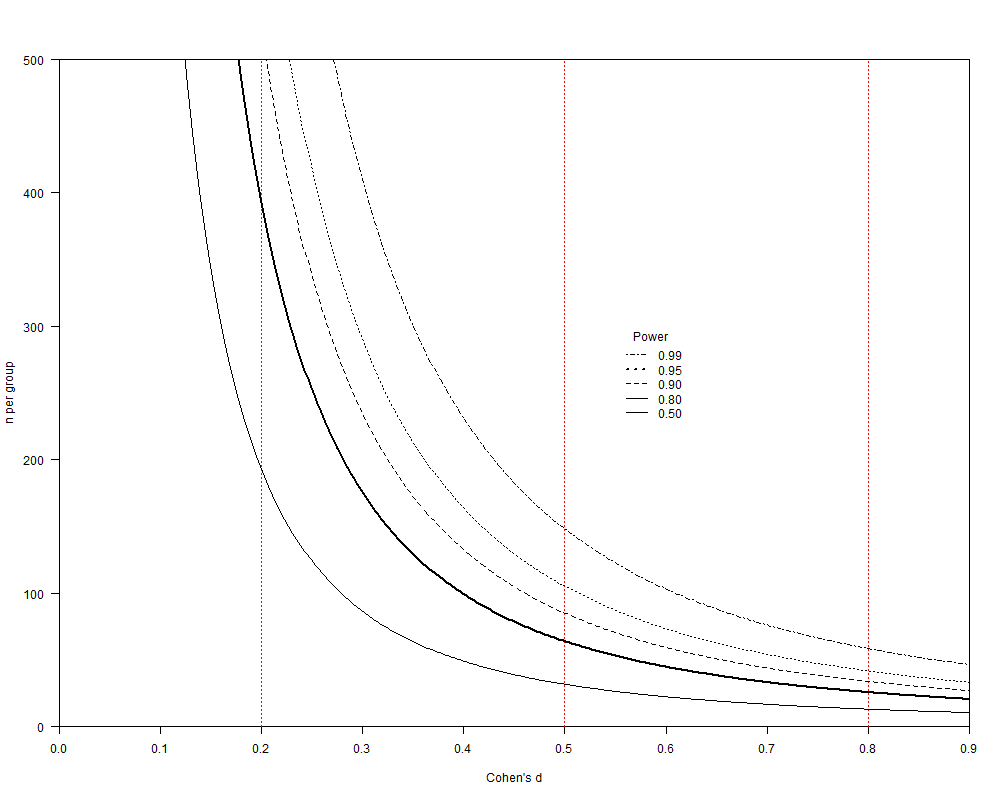
\includegraphics[height=0.8\textheight, trim = 0in 0in 0in 0.5in , clip]{images/power}
\end{center}

}

\frame{

\frametitle{Power in Legislative Experiments}

\begin{itemize}\itemsep1em
\item<2-> Legislatures are small!!!

\item<3-> Because $N$ is fixed, limited capacity to increase $n$, so power has to be maximized by:

	\begin{itemize}
	\item Reducing item variance in outcome measures
	\item Studying treatments with bigger effects
	\item Expanding scope of studies
	\item Creative research design
	\end{itemize}

\end{itemize}

}


\questions


\frame{}

\section[Experimental Design]{From Theory to Experimental Design}
\frame{\tableofcontents[currentsection,subsubsectionstyle=hide]}
% deriving hypotheses from theory and manipulations from hypotheses


\frame{

\frametitle{Experimental Hypothesis Testing}

\begin{itemize}\itemsep1em
\item From theory, we derive testable hypotheses\\

	\begin{itemize}
	\item Hypotheses are expectations about differences in outcomes across levels of a putatively causal variable
	\item In an experiment, an hypothesis must be testable by an SATE
	\end{itemize}

\item The experimental manipulations induce variation in the causal variable that enable tests of the hypotheses
\end{itemize}

}


\frame{

\frametitle{{\normalsize Example: Framing and Attention\footnote{Walgrave, Sevenans, Van Camp, Loewen (2017) -- ``What Draws Politicians' Attention? An Experimental Study of Issue Framing and its Effect on Individual Political Elites''}}}

\small

\begin{itemize}
\item Theory: Presentation of information affects politicians' attention
\item Hypothesis:
	\begin{itemize}\footnotesize
	\item Information framed as a conflict draws more attention from political elites than information not framed as a conflict.
	\end{itemize}
\item Manipulation:
	\begin{itemize}\footnotesize
	\item Control group: Presentation of headline information
	\item Treatment group: Same information presented as conflict
	\end{itemize}
\item Outcome:
	\begin{itemize}
	\item How likely are legislators to read full article
	\end{itemize}
\end{itemize}

}


\frame{

\frametitle{{\normalsize Ex.: Presence/Absence}}

\small

\begin{itemize}\itemsep0.5em
\item Theory: Legislators vote in line with constituents' preferences
\item Hypothesis: Exposure to a poll of constituent views shifts legislative votes.
\item Manipulation:
	\begin{itemize}\small 
	\item Control group receives no polling information. 
	\item Treatment group receives a letter containing polling information.
	\end{itemize}
\item Outcome:
	\begin{itemize}
	\item How legislators vote on relevant piece of legislation
	\end{itemize}
\end{itemize}

}


\frame{

\frametitle{{\normalsize Ex.: Levels/doses}}

\small

\begin{itemize}\itemsep-0.2em
\item Theory: Legislators vote in line with constituents' preferences
\item Hypothesis: Exposure to a poll of constituent views shifts legislative votes.
\item Manipulation:
	\begin{itemize}\small 
	\item Control group receives no polling information. 
	\item Treatment group 1 receives a letter containing polling information.
	\item Treatment group 2 receives two letters containing polling information.
	\item etc.
	\end{itemize}
\item Outcome:
	\begin{itemize}
	\item How legislators vote on relevant piece of legislation
	\end{itemize}
\end{itemize}

}


\frame{

\frametitle{{\normalsize Ex.: Qualitative variation}}

\small

\begin{itemize}
\item Theory: Legislators vote in line with constituents' preferences
\item Hypothesis: Exposure to a poll of constituent views shifts legislative votes.
\item Manipulation:
	\begin{itemize}\small 
	\item Control group receives no polling information. 
	\item Treatment group 1 receives a letter containing polling information suggesting public support.
	\item Treatment group 2 receives a letter containing polling information suggesting public opposition.
	\end{itemize}
\item Outcome:
	\begin{itemize}
	\item How legislators vote on relevant piece of legislation
	\end{itemize}
\end{itemize}

}

\frame{

\frametitle{Treatments Test Hypotheses!}

\begin{itemize}\itemsep0.5em
\item<2-> Derive experimental design from hypotheses
\item<3-> Experimental ``factors'' are expressions of hypotheses as randomized groups
\item<4-> What intervention each group receives depends on hypotheses
	\begin{itemize}
	\item presence/absence
	\item levels/doses
	\item qualitative variations
	\end{itemize}
\end{itemize}

}

\frame{

\begin{center}
\large But how do we know that the experiment worked?
\end{center}

}


\frame{

\begin{quote}\large
The best criterion for evaluating the quality of an experiment is whether it manipulated the intended independent variable and controlled everything else by design.
\end{quote}
\onslide<2->{\small\hspace{5em} --Thomas J. Leeper (18 August 2017)}

}

\frame{

\frametitle{How do we know we manipulated what we think we manipulated?}

\small

\begin{itemize}
\item<2-> Outcomes are affected consistent with theory
\item<3-> Before the study using \textit{pilot testing} (or \textit{pretesting})
\item<4-> During the study, using \textit{manipulation checks}
\item<5-> During the study, using \textit{placebos}
\item<6-> During the study, using \textit{non-equivalent outcomes}
\end{itemize}

\only<6->{These may not all be possible and all are incompletely informative.}
}

\frame{

\frametitle{How do we know we controlled what we think we controlled?}

\small

\begin{itemize}
\item<2-> Measure characteristics across groups to test for \textit{covariate balance}, but imbalance does not necessarily imply experimental failure

\item<3-> In field experiments, measure whether legislators were actually treated (i.e., actually received and \textit{complied} with their assigned treatment)

\item<4-> Measure whether there were spillovers between experimental conditions if possible
\end{itemize}

\only<5->{These may not all be possible and all are incompletely informative.}
}

\questions


\frame{}




\section[Paradigms]{Paradigms and Examples}
\frame{\tableofcontents[currentsection,subsubsectionstyle=hide]}

\frame{

\frametitle{Three Major Paradigms}

\begin{enumerate}\itemsep1em
\item Field Experiments

	\begin{itemize}\small
	\item Ex. Broockman (2013) -- ``Black Politicians Are More Intrinsically Motivated to Advance Blacks' Interests''
	\end{itemize}

\item Survey Experiments

	\begin{itemize}\small
	\item Ex. Renshon, Yarhi-Milo, and Kertzer (2016) -- ``Democratic Leaders, Crises and War: Paired Experiments on the Israeli Knesset and Public''
	\end{itemize}

\item Simulations

	\begin{itemize}\small
	\item Ex. Frechette, Kagel, Lehrer (2003) -- ``Bargaining in Legislatures: An Experimental Investigation of Open versus Closed Amendment Rules''
	\end{itemize}

\end{enumerate}

}


\frame{

\frametitle{Paradigm 1: Field Experiments}

\small

\begin{itemize}\itemsep0.5em
\item Basic idea: randomly expose legislators \textit{in situ} to some experience and measure an outcome that might be affected by it

\item Two ``flavours''

	\begin{enumerate}
	\item Orchestrated by the researcher(s)
	\item ``Natural'' experiments not orchestrated by the researcher(s)
	\end{enumerate}

\item Tend to be simple in terms of design due to practical difficulty of exposing legislators' to treatment and measuring outcomes

\item ``Natural'' experiments are limited by randomized institutions being rare (e.g., committee assignments, office locations, proposal rights/order, etc.)
\end{itemize}

}


\frame{

\frametitle{Paradigm 1: Field Experiments}

\begin{itemize}\itemsep0.5em

\item Example of Flavour A

	\begin{itemize}
	\item Broockman (2013)
	\item Treatment: Form of contact from a prospective constituent
	\item Outcome: Whether a response is received
	\item Effect: Difference in response rates by treatment
	\end{itemize}

\item Example of Flavour B

	\begin{itemize}
	\item Kellermann, Shepsle (2009)
	\item Treatment: Freshmen legislators are randomly ordered in determining committee assignments
	\item Outcome: Various metrics of leadership and legislative activity
	\item Effect: Difference in those outcomes between higher- and lower-ranked legislators
	\end{itemize}

\end{itemize}
}

\frame{

\frametitle{Paradigm 2: Survey experiments}

\begin{itemize}\itemsep1em
\item Basic idea: conduct interviews with legislators (in-person or through another mode), where features of questionnaire are randomized

\item Recruiting legislators into interviews tends to be extremely difficult, thus:

	\begin{itemize}
	\item Almost unavoidably underpowered 
	
	\item Can only study legislators who agree to participate

	\item Necessarily simplistic designs with treatment and outcome measured in a single interview\footnote{Can be generalized to allow field treatments with survey measures, or survey treatments with field measures}
	
	\item Survey experiments on legislators tend to be rare
	\end{itemize}

\end{itemize}

}

\frame{

\frametitle{{\normalsize Paradigm 2: Survey Experiments}}

\small

Example:

\begin{itemize}\itemsep0.5em

\item Butler and Dynes (2016)

\item Treatment: State legislators completing a survey read a hypothetical constituent letter with varying stated opinions

\item Outcome: Measures of perceptions of constituent characteristics (e.g., knowledge)

\item Effect: Difference in perceptions b/w constituents with similar/dissimilar views to legislator

\end{itemize}
}


\frame{

\frametitle{Paradigm 3: Simulations}

\small

\begin{itemize}\itemsep1em
\item Basic idea: Derive theoretical expectations about legislative behavior and test those predictions in a \textit{stylized} legislative context using non-legislators as participants

\item These are historically much more common than paradigms 1 or 2

\item Unique considerations:

	\begin{itemize}
	\item Tend to be based in formal theories of legislatures
	\item Sample sizes limited by resources
	\item Historically in labs, but increasingly common online
	\item Tend to lack face validity given context and participants
	\end{itemize}
\end{itemize}

}


\frame{

\frametitle{Paradigm 3: Simulations}

Example:

\begin{itemize}\itemsep1em

\item Wilson (1986)

\item Treatment: ``Legislators'' vote under open or closed amendment rules

\item Outcome: The final ``policy'' adopted by the ``legislature''

\item Effect: Difference in ``policy'' adopted by the legislature

\end{itemize}
}


\questions

\frame{

\frametitle{15-minute Activity!}

\begin{enumerate}

\item Divide into three groups

\item<2-> Groups discuss one of the texts:

	\begin{itemize}
	\item Group 1: Broockman (2013)
	\item Group 2: Renshon, Yarhi-Milo, and Kertzer (2016)
	\item Group 3: Frechette, Kagel, Lehrer (2003)
	\end{itemize}

\item<3-> Discuss:

	\begin{itemize}
	\item What is the experiment? How does it work?
	\item What do the authors find? What is the effect?
	\item What are the practical challenges/issues raised?
	\end{itemize}
\end{enumerate}

}

\frame{}


\frame{

\frametitle{Activity!}

\begin{itemize}\itemsep0.5em
\item How do we know if an experiment is any good?
\item Write for 3 minutes to yourself
\item<2-> Talk with a partner for about 3 minutes
\item<2-> Try to develop some criteria that allow you to evaluate ``what makes for a good experiment?'' 
\end{itemize}

}

\section[Challenges]{Challenges of Legislative Experiments}
\frame{\tableofcontents[currentsection]}

\frame{

\frametitle{Many Challenges,\\Too Little Time}

\begin{enumerate}\itemsep1em
\item Nonresponse and Noncompliance

\item Spillover

\item What can be randomized?

\item Ethics
\end{enumerate}

}


% Nonresponse and Noncompliance
\frame{
\frametitle{Nonresponse}

\begin{itemize}\itemsep1em

\item In survey experiments, nonresponse may introduce challenges:

	\begin{itemize}
	\item Underpowered designs
	\item Response biases that affect generalizability
	\item Nonresponse may be due to treatment
	\item Nonresponse may be due to attrition
	\end{itemize}

\item The only way to avoid nonresponse is to try to incentivize response or minimize effort involved in a study

\item Real risk: more surveys might create common pool resource problems!
\end{itemize}

}


\frame{
\frametitle{Compliance}

\small

\begin{itemize}\itemsep0.5em
\item Compliance is when individuals receive and accept the treatment to which they are assigned, as opposed to:
	\begin{itemize}
	\item Receiving the wrong treatment (cross-over)
	\item Failing to receive any treatment 
	\end{itemize}
\item This causes problems for our analysis because factors other than randomization explain why individuals receive their treatment

\item Possible responses to noncompliance:
	\begin{itemize}
	\item ``As treated'' analysis
	\item ``Intention to treat'' analysis
	\item Estimate a LATE
	\end{itemize}
\end{itemize}
}

\frame{
\frametitle{Analyzing Noncompliance}

\small

\begin{itemize}\itemsep0.5em
\item If noncompliance only occurs in one group, it is \textit{asymmetric} or \textit{one-sided}

\item We can ignore non-compliance and analyze the ``intention to treat'' effect, which will underestimate our effects because some people were not treated as assigned: $ITT = \overline{Y}_1 - \overline{Y}_0$

\item<2-> We can use ``instrumental variables'' to estimate the ``local average treatment effect'' (LATE) for those that complied with treatment: $LATE = \frac{ITT}{\% Compliant}$

\item<3-> If noncompliance is symmetric, analysis much more complicated.
\end{itemize}
}

\questions


% Spillover
\frame{

\frametitle{Spillover}

\begin{itemize}\itemsep1em
\item A key assumption of experimental analysis is that units are \textit{independent}

\item This assumption may be implausible in legislatures because units are in regular communication and may ``share'' some of their treatment with others in the group

\item What can be done?

	\begin{itemize}
	\item Try to avoid it by design!
	\item Exclude individuals affected by spillovers, if observable
	\item More complicated procedures
	\end{itemize}

\end{itemize}

}

% What can be randomized?
\frame{

\frametitle{What can be randomized?}

\small

\begin{itemize}\itemsep0.5em
\item In theory almost anything can be randomized, but not everything

	\begin{itemize}
	\item Intrinsic characteristics
	\item Institutional features (outside of simulations)
	\item Contextual factors
	\end{itemize}

\item Anything that is ``information-like'' can easily and obviously be randomized\footnote{Messages, contact, personal interactions, etc.}

\item If you want to study factors that are not information-like:

	\begin{itemize}
	\item Look for ``natural'' experiments
	\item Run simulations
	\item Run field or survey experiments that attempt to modify the \textit{salience} of those factors
	\end{itemize}
\end{itemize}

}


% Ethics
\frame{

\frametitle{Research Ethics}

\begin{itemize}\itemsep1em
\item Researchers have obligations to attempt to:
	\begin{itemize}
	\item minimize risk to participants
	\item to maximize benefits to human knowledge
	\item to protect the privacy of personal data
	\item to fairly and objectively report their research
	\end{itemize}
\item<2-> These rules vary to some extent across contexts
\item<3-> But a major question is whether these ``standard'' ethical rules also apply to politicians. What do you think?
\end{itemize}

}

\questions


\frame{}





\section{Student Presentations}
\frame{\tableofcontents[currentsection,subsubsectionstyle=hide]}

\frame{

\begin{center}
\Large

Student presentations!
\end{center}

}



\frame{}

\section{Conclusion}
\frame{\tableofcontents[currentsection,subsubsectionstyle=hide]}

\againframe<5>{learningoutcomes}

\frame{

\frametitle{In Conclusion}

\begin{itemize}\itemsep1em
\item Experiments are mostly about design, not analysis

\item Experiments are underutilized in legislative contexts, in part because conducting them effectively is extremely difficult

\item This means that careful but often simple design can generate potentially powerful and novel insights into legislative behavior
\end{itemize}

}

\end{document}
